\clearpage
{\bfseries ҒТАХР 50.47.29}\hfill
\hfill {\bfseries \href{https://doi.org/10.58805/kazutb.v.2.19-113}{https://doi.org/10.58805/kazutb.v.2.19-113}}

\sectionwithauthors{Тулегулов А.Д., АкишевК.М., Юрков Н.К., Островерхов Д.}{ТАУ-КЕН ӨНЕРКӘСІБІНЕ АРНАЛҒАН ДИСПЕТЧЕРЛІК-ТАЛДАМАЛЫҚ ЖҮЙЕ}

\begin{center}
{\bfseries А.Д. Тулегулов\textsuperscript{1*}, К.М.
Акишев\textsuperscript{1}, Н.К. Юрков\textsuperscript{2}, Д.
Островерхов\textsuperscript{3}}

\textsuperscript{1}Қазақ технология және бизнес университеті, Астана,
Қазақстан,

\textsuperscript{2}Пенза мемлекеттік университеті, Пенза, Ресей
Федерациясы

\textsuperscript{3}Берлин техникалық университеті, Берлин, Германия,

tad62@ya.ru
\end{center}

\hspace{1.5em} Жұмыста тау-кен өнеркәсібіне арналған диспетчерлік-аналитикалық жүйені
қолданудың өзектілігі көрсетілген. Эксперименттік зерттеулердің мақсаты
тау-кен өнеркәсібі үшін диспетчерлік-аналитикалық жүйені қолдану
әдістемесін әзірлеу болып табылады. Соңғы онжылдықтарда тау-кен
металлургия кешендерін басқаруды басқаруды автоматтандырудың әртүрлі
жүйелері өте белсенді дамып келеді, бұл өз кезегінде автоматика және
диспетчерлеу жүйелерінің элементтері мен құрылғыларын таңдауға жоғары
талаптар қояды.

\hspace{1.5em} {\bfseries Түйінді сөздер:} диспетчерлік-талдамалық жүйе, әдістеме, тау-кен
өнеркәсібі, тау-кен металлургия кешені, бақылау аппаратурасы, басқару
жүйелері, датчиктер, метан

\begin{center}
{\large\bfseries ДИСПЕТЧЕРСКО-АНАЛИТИЧЕСКАЯ СИСТЕМА ДЛЯ ГОРНОДОБЫВАЮЩЕЙ ПРОМЫШЛЕННОСТИ}

\vspace{1em}

{\bfseries А.Д. Тулегулов\textsuperscript{1*}, К.М.
Акишев\textsuperscript{1}, Н.К. Юрков\textsuperscript{2}, Д.
Островерхов\textsuperscript{3}}

\textsuperscript{1}Казахский университет технологии и бизнеса,

\textsuperscript{2}Пензенский государственный университет, Пенза,
Российская Федерация,

\textsuperscript{3}Берлинский технический университет, Берлин, Германия,

tad62@ya.ru
\end{center}

\hspace{1.5em} В работе показана актуальность применения диспетчерско-аналитической
система для горной промышленности. Целью экспериментальных исследований
является разработка методологии применения диспетчерско-аналитической
системы для горной промышленности. В последние десятилетия очень активно
развиваются различные системы автоматизации контроля управления
горно-металлургическими комплексами, что в свою очередь предъявляет
более высокие требования к выбору элементов и устройств систем
автоматики и диспетчеризации.

\hspace{1.5em} {\bfseries Ключевые слова:} диспетчерско-аналитическая система,
методология, горная промышленность, горно-металлургический комплекс,
аппаратура контроля,, системы управления, датчики, метан.

\begin{center}
{\large\bfseries DISPATCH AND ANALYTICAL SYSTEM FOR THE MINING INDUSTRY}

\vspace{1em}

{\bfseries A.D.Tulegulov\textsuperscript{1*}, K.M.
Akishev\textsuperscript{1}, N.K. Yurkov\textsuperscript{2}, D.
Ostroverkhov\textsuperscript{3}}

\textsuperscript{1}Kazakh University of Technology and Business, Astana.
Kazakhstan,

\textsuperscript{2}Penza State University, Penza, Russia,
\textsuperscript{3}Technical University, Berlin, Germany,

tad62@ya.ru
\end{center}

\hspace{1.5em} The paper shows the relevance of the use of a dispatching and analytical
system for the mining industry. The purpose of the experimental research
is to develop a methodology for the use of a dispatching and analytical
system for the mining industry. In recent decades, various automation
systems for control control of mining and metallurgical complexes have
been actively developing, which in turn imposes higher requirements on
the selection of elements and devices of automation and dispatching
systems.

\hspace{1.5em} {\bfseries Keywords:} dispatch and analytical system, methodology, mining
industry, mining and metallurgical complex, control equipment, control
systems, sensors, methane.

\vspace{1em}

\begin{multicols}{2}
{\bfseries Кіріспе.} Тау-кен өндірісін автоматтандыру-қауіпсіздікті
арттырудың жолы. Тау - кен өндірісін автоматтандыру-консервативті
салалардың бірі. Көптеген кезеңдерде өндірістік тізбектер бірнеше
онжылдықтар бұрын болған сияқты ескі әдіспен жұмыс істейді. Өндіруші
кәсіпорындарды жаңғырту - олардың тиімділігі мен табыстылығын арттыру
ғана емес, сонымен қатар қауіпсіздік мәселесі.

Тау-кен өнеркәсібінің технологиялық процестерін автоматтандыру бірқатар
мақсаттарға қол жеткізу үшін жүзеге асырылады, мысалы, өндірудің
өнімділігін арттыру( шикізат көлемі мен сапасы), шығындарды азайту,
әсіресе жер асты және жер үсті жұмыстарының энергия тиімділігі
көрсеткіштерін жақсарту, бұрын қолмен орындалған немесе бақыланатын
технологиялық процестерді механикаландыру арқылы штаттық құрамды
оңтайландыру, қауіпсіздік стандарттарын жақсарту. авариялық жағдайларды
уақтылы болдырмау, өндірістік тізбектің барлық учаскелерінде жабдықтың
жай-күйін үнемі өзін-өзі диагностикалау {[}1{]}.

Тау-кен-шахта жабдықтарына және автоматика және телемеханика жүйелеріне
қойылатын заманауи талаптарды ескере отырып, алдын ала сынақтар
жүргізуді, ақпаратты беру аппаратурасы (АПИ) мен түрлі түрлендіргіштер
негізінде жүйені тәжірибелік пайдалану мен қабылдау сынақтарын көздейтін
жаңа жұмыс жобалары әзірленуде. Жүйені сынау және пайдалану бекітілген
шахталық сынақ бағдарламасы мен әдістемесіне сәйкес шахтаның нақты
жағдайларында көзделеді.

{\bfseries Материалдары мен зерттеу әдістемесі.} Осы ғылыми мақалада
зерттеу объектісі ретінде "Қазақстан" шахтасы қарастырылады. Бақылау
объектілері ретінде шахтаның шешімі бойынша жобаның құрамына № 2 және №
5 қазу учаскелері енгізілді. Қазба учаскелерінде жүйе келесі параметрлер
туралы орталық диспетчерлік пунктке (ЦДП) ақпаратты бақылауды және
беруді қамтамасыз етеді:

- жалпы шығатын желдету ағындарындағы және келіп түсетін жаңа
ағындардағы ауаның жылдамдығы (шығысы);

- ПБ телеөлшеу қарастырылатын қазу учаскесінің нүктелеріндегі метан
концентрациясы.

Жүйенің техникалық құралдарының құрамына ақпаратты іріктеу құралдары,
Ақпаратты беру аппаратурасы және беттік есептеу кешені кіреді. Ақпаратты
іріктеу құралы ретінде жүйеде "МЕТАН" кешенінің ДМТ-4 метан
концентрациясының сериялық датчиктері және депрессия мен ауа
жылдамдығының ПДС-1 түрлендіргіштері қолданылады. Көрсетілген датчиктер
мен түрлендіргіштерден ақпаратты берудің техникалық құралы ретінде АПИ
аппаратурасы пайдаланылады. АПИ аппаратурасы ПДО - да орналасқан УПК
қабылдау-командалық құрылғысынан, РГ топтық таратқыштарынан және бақылау
объектілерінде орнатылатын ПТИ телеөлшеу түрлендіргіштерінен тұрады.
Беттік есептеу кешенінің құрамына IBM класындағы екі компьютер кіреді
(біреуі сауалнама режимінде, екіншісі ақпаратты жинақтау және өңдеу
режимінде), жұптастыру құрылғысы (УC), қабылдау-командалық құрылғы
(УПК), AПИ аппаратурасы {[}2-3{]}.

Осы жобада пайдаланылатын жаңа аппаратура туралы негізгі мәліметтер,
техникалық деректер, құрылғысы және жұмыс принципі, монтаждау және
техникалық қызмет көрсету жөніндегі нұсқаулар және басқа да мәліметтер
мынадай құжаттарда келтірілген:

- "УХЛ5 АПИ ақпарат беру аппаратурасы. АПИ 00.000 РЭ эксплуатация
жөніндегі Нұсқаулық";

- "Депрессия және ауа жылдамдығы ПДС-1 УХЛ5 түрлендіргіші. ПДС пайдалану
жөніндегі Нұсқаулық-1 00.000 РЭ";

- "АПИ аппаратурасын IBM типті ДК-мен жұптастыру құрылғысы. Пайдалану
жөніндегі Нұсқаулық, УС 00.000 РЭ";

- Орталықтандырылған аэрогазды бақылау жүйесі (АГК). Оператор
басшылығы";

- "Complex элементтеріне арналған қысқаша анықтамалық нұсқаулық".

\emph{Аппаратураның құрамы және орналасуы}

Жүйенің техникалық құралдарының құрамына (1-сурет) жер үсті есептеу
кешені және өндіру учаскелерін аэрогаздық бақылау құралдары кіреді.

{\centering
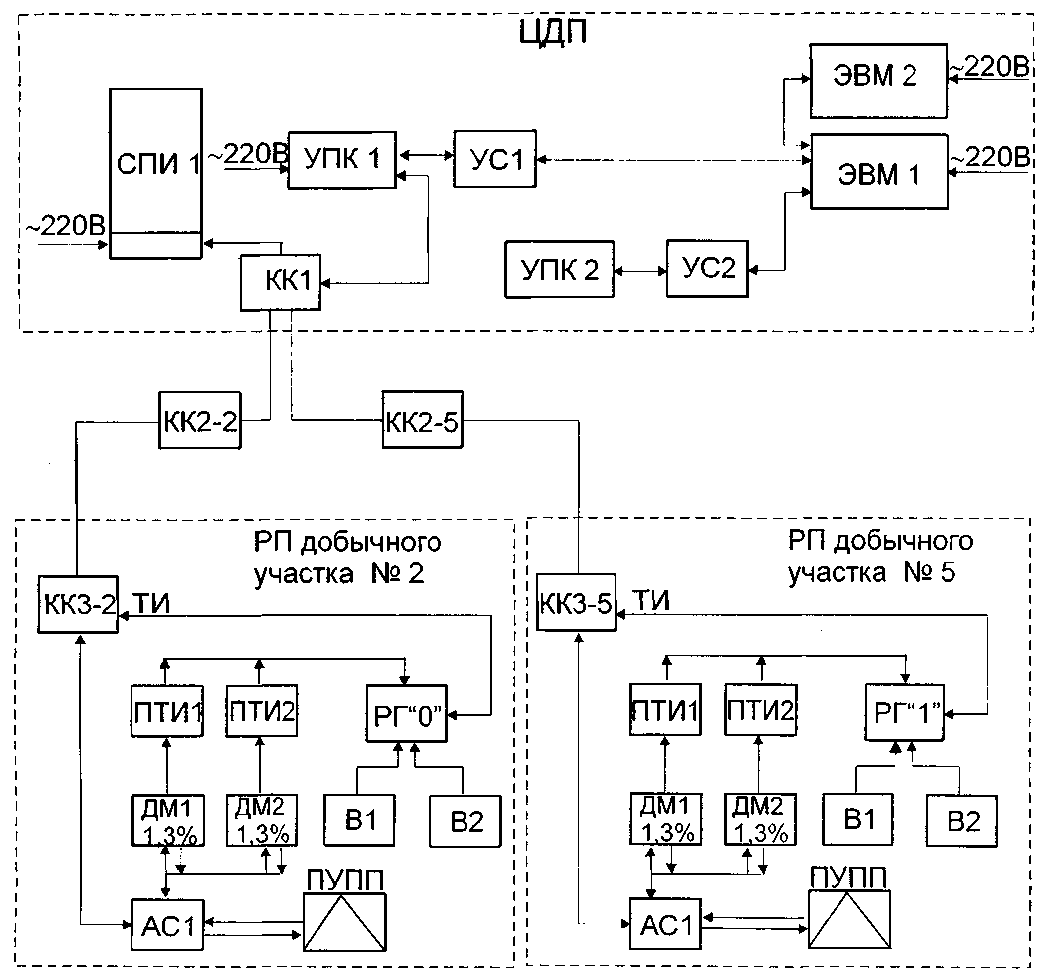
\includegraphics[width=\columnwidth]{image69}
\captionof*{figure}{Сурет 1 - "Қазақстан" шахтасының автоматика және телемеханика жүйесінің құрылымдық схемасы}}

ЦДП - орталық диспетчерлік пункт; СПИ 1 - "Метан" кешенінің тірегі;
УПК1, УПК2-қабылдау-командалық құрылғы; УС1, УС2-түйісу құрылғысы; ЭЕМ1,
ЭЕМ2 - IBM типті дербес микро ЭЕМ; РГО", РГТ - топтық дистрибьютор;
ПТИ1, ПТИ2-телеөлшеу түрлендіргіші; В1, В2 - депрессия және ауа
жылдамдығын түрлендіргіш ПДС - 1; ДМ1, ДМ2-метан датчигі ДМТ; АС1 -
"Метан" кешенінің дабыл аппараты; ПУПП-жылжымалы учаскелік жерасты
қосалқы станциясы; КК1-бөлу шкафы; КК2, ККЗ - кабельдік қорап

Жүйенің техникалық құралдарының құрамы:

1. Беттік есептеу кешені IBM класындағы екі компьютерден тұрады (біреуі
сауалнама режимінде, екіншісі ақпаратты жинақтау және өңдеу режимінде),
екі УС, екі УПК және кабельді сымдарға арналған шкафтар (кросс).
Кешеннің барлық құралдары шахтаның ЦДП үй-жайында АГК операторының
арнайы ұйымдастырылған жұмыс орнында орналасады. Оператордың үй-жайының
өлшемдеріне байланысты есептеу кешенінің құралдары ұзындығы бойынша
немесе ұтымды конфигурацияның бірнеше кестесінде орналасуы мүмкін.

%% \end{multicols}

%% \begin{figure}[H]
%%     \centering
%%     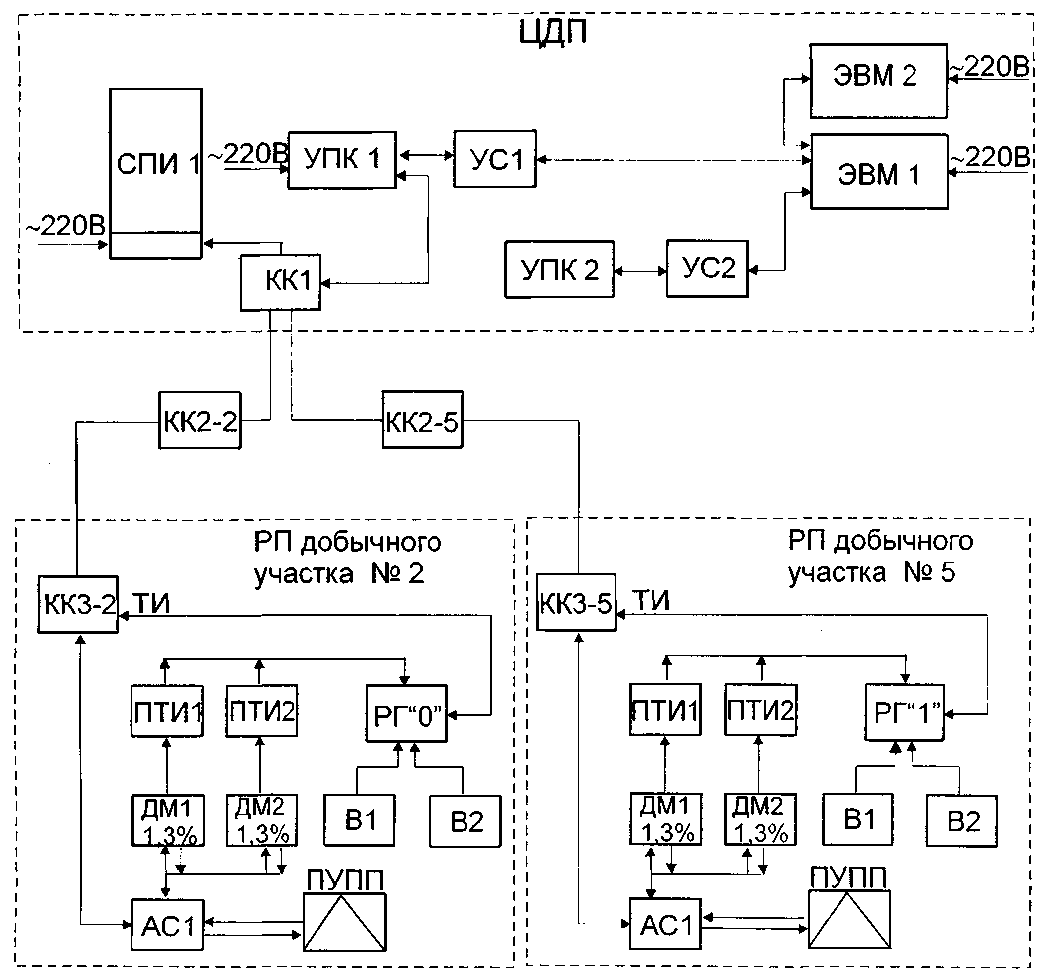
\includegraphics[width=0.6\textwidth]{image69}
%%     \caption*{Сурет 1 - "Қазақстан" шахтасының автоматика және телемеханика жүйесінің құрылымдық схемасы}
%% \end{figure}

%% \begin{multicols}{2}

1-суреттен көріп отырғаныңыздай, ақпаратты беру аппаратурасының бір
жиынтығы (УПК1, УС1) және екі компьютер жұмыс режимінде (қосылған), ал
екінші (УПК2, УС2) компьютерге қосылған, бірақ өшірулі күйде (резервте).
Жұмыс УПК1-ден байланыс желісі (төрт сым) оператор үй-жайының кроссына
(КК1) кіреді, содан кейін екі жолға бөлінеді. Бір байланыс желісі екі
клеткалы оқпан бойымен КК2-2 жерасты кабель қорабына, содан кейін №2
өндіру учаскесіне өтеді. Екінші байланыс желісі жаңа екі клеткалы бөшке
арқылы КК2-5 жерасты қорабына, содан кейін №5 өндіру учаскесіне өтеді.

2. Өндіру учаскелеріндегі аэрогазды бақылаудың техникалық құралдарының
құрамына "МЕТАН" кешенінің сериялы шығарылатын аппаратурасының ДМТ-4
метан концентрациясының датчиктері, ПДС-1 депрессия және ауа
жылдамдығының түрлендіргіштері, ПТИ телеөлшеу түрлендіргіштері және
топтық дистрибьюторы кіреді.

3. Шахтаның техникалық кеңесінің хаттамасына сәйкес бақылау жүйесіне №2
және №5 өндіру учаскелері енгізіледі. Өндіру учаскелеріндегі климаттық
және пайдалану шарттары төменде келтірілген.

№ 2 өндіру учаскесі-Лава 233-Д11-В:

- өңделетін қабат-Д11;

- желдету схемасы-тікелей, төмен түсетін, сергітетін;

- желдету қазбаларының қимасы, м:

- шегіну (вент. пром. штрек 233-Д11-В) - 8,6; жаңару (конв. пром. штрек
233-Д11-В) - 11,0; Шығыс учаскесі (конв. пром. штрек 233-Д11-В) - 9,3;

- ауа шығыны, м\textsuperscript{3}/мин: кіріс - 773; жаңарту - 1050;
Шығыс учаскесі-1693.

Төменде 2-суретте "Қазақстан" шахтасының кабельдік байланыс желілерінің
құрылымдық сызбасы көрсетілген.
\end{multicols}

\begin{figure}[H]
    \centering
    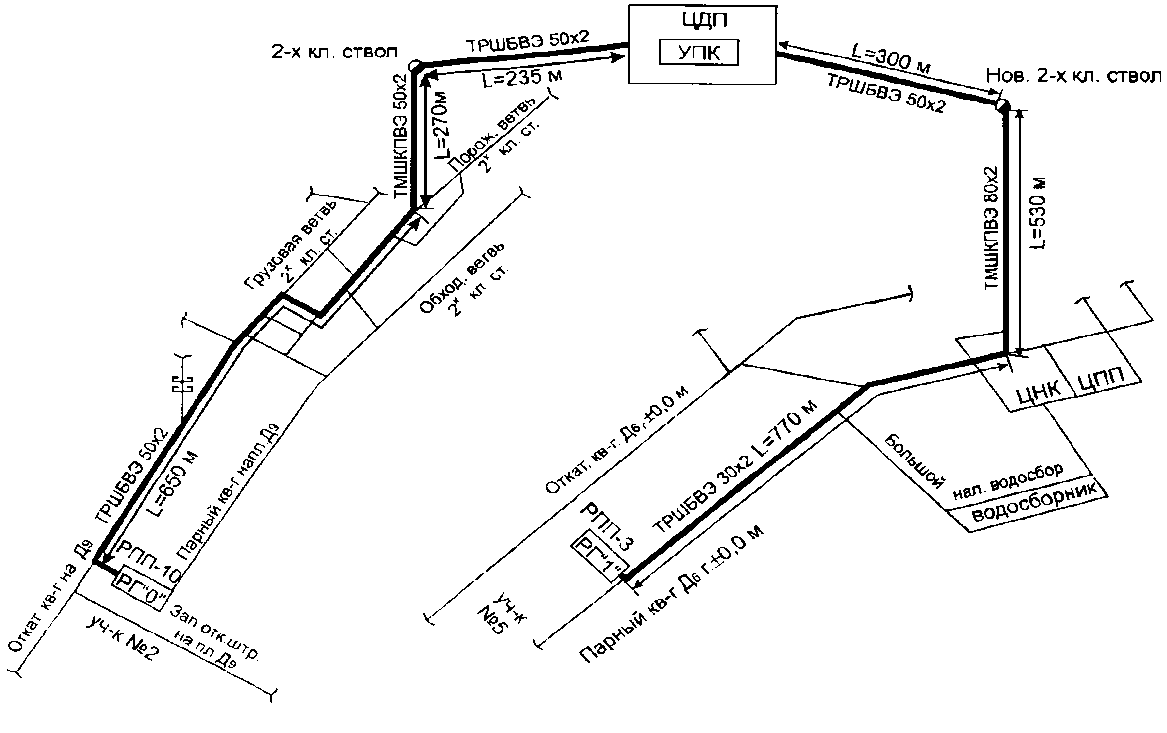
\includegraphics[width=\textwidth]{image70}
    \caption*{Сурет 2- "Қазақстан" шахтасының кабельдік байланыс желілерінің құрылымдық сызбасы}
\end{figure}

3-суретте "Қазақстан" шахтасының орталық диспетчерлік пунктінде жүйе
аппаратурасының орналасу сызбасы көрсетілген. Бұл схемада жұмыс жиынтығы
ретінде УС1 жұптастыру құрылғысы, қабылдау-командалық upc1 құрылғысы
қолданылады. Резервтік жинақ ретінде УС2 жұптастыру құрылғысы,
қабылдау-командалық УПК2 құрылғысы пайдаланылды. 1-монитор 1-есептеу
кешенінде, ал 2-монитор 2-есептеу кешенінде қолданылады.

\begin{figure}[H]
    \centering
    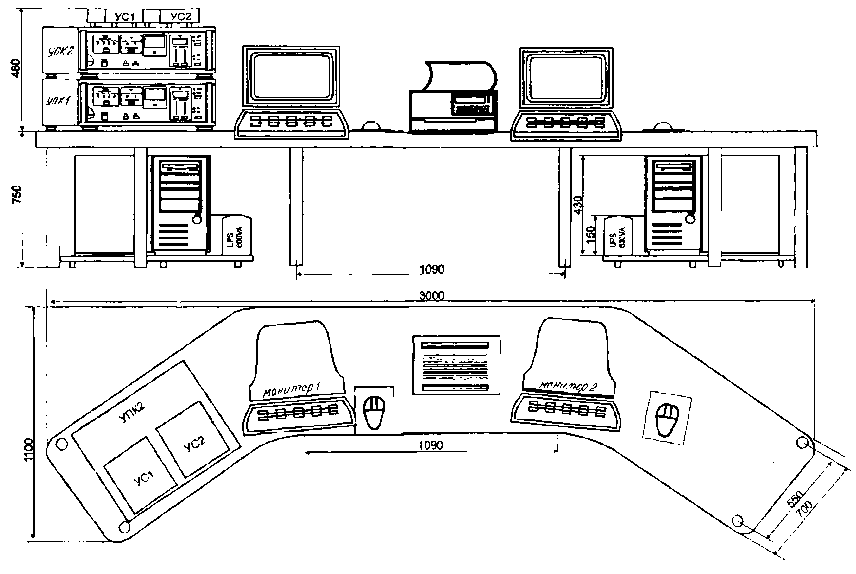
\includegraphics[width=0.7\textwidth]{image71}
    \caption*{Сурет 3- "Қазақстан" шахтасының орталық диспетчерлік пунктінде жүйе
аппаратурасының орналасу сызбасы}
\end{figure}

\begin{longtable}[]{@{}
  >{\raggedright\arraybackslash}p{(\columnwidth - 6\tabcolsep) * \real{0.2503}}|
  >{\raggedright\arraybackslash}p{(\columnwidth - 6\tabcolsep) * \real{0.3829}}|
  >{\raggedright\arraybackslash}p{(\columnwidth - 6\tabcolsep) * \real{0.0737}}|
  >{\raggedright\arraybackslash}p{(\columnwidth - 6\tabcolsep) * \real{0.2932}}@{}}
\caption*{Кесте 1."Қазақстан" шахтасының ЦДП-да орнатылатын жүйе аппаратурасының тізбесі} \\
\toprule\noalign{}
\endhead
\bottomrule\noalign{}
\endlastfoot
Атауы & Түрі, маркасы & Саны & Жалпы өлшемдер \\
Монитор & Studioworks 563 N & 2 & 370\(\)410\(\)380 \\
Тышқан & Midi Tower АТХ 300 W & 2 & 180\(\)430\(\)440 \\
Аудио динамиктер & Genius Net Scroll+USB & 2 & 65\(\)40\(\)110

230\(\)1 80 коврик \\
Желілік қосқыш және қуат көзі & COMPEX PS 2208/A/D Fast Ethernet Pocket
Switch 8 port 10/100 Mbits & 1 & 210\(\)50\(\)190 65\(\)30\(\)150 \\
Үздіксіз қуат көзі & UPS 600VA Power MAN Back PRO 600 & 2 &
90\(\)150\(\)400 \\
Желілік сүзгі & Vertor SOLO (4-х розеток) & 2 & 200\(\)40\(\)60 \\
Қабылдау-командалық құрылғы & УПКАПИ01.000 & 2 & 480\(\)170\(\)500 \\
Жұптастыру құрылғысы & УС 00.000 & 2 & 185\(\)65\(\)190 \\
\end{longtable}

\begin{multicols}{2}
Жобаның тиімділігін бағалаудың ең дұрыс әдісі ретінде таңдалған
жабдықтың оңтайлы жұмыс режимдерін анықтау үшін технологиялық процесті
модельдеу болып табылады.

{\bfseries Негізгі нәтижелер}

Жүргізілген зерттеулердің сенімділігі үшін біз технологиялық процестің
негізгі параметрлерінің нақты мәндерін қолданамыз:

- ауа жылдамдығы, м/с: кіріс-1,5; жаңарту-1,6; шығыс учаскесі - 3,0;

- салыстырмалы метанобильділік, м\textsuperscript{3}/мин - 2,82;

- қоршаған орта температурасы, °С - 16-20;

- салыстырмалы ылғалдылық, \% - 98 дейін;

- атмосфералық қысым, кПа - 92-98;

- шаңдану, мг/м\textsuperscript{3}-67.

№ 5 өндіру учаскесі-Лава 234-Д6-1В.

- пайдаланылған қабат-Д6;

- желдету схемасы-тікелей, төмен, артқы жағымен;

- желдеткіш қазбаларының қимасы, м:

келіп түскен (конв. пром. штрек 224-Д6-1 - В) - 9,7; жаңару (конв.
пром. штрек 234-Д6-1-В) - 14,8; Шығыс учаскесі (монтаждау камерасы
244-Д6-1-В) - 11,9;

- ауа шығыны, м\textsuperscript{3}/мин: кіріс - 577; сергіту-665;

Шығыс учаскесі -1241;

- ауа жылдамдығы, м/с: кіріс-1,0; жаңарту-0,75; шығыс учаскесі -1,7;

- метанобильділік, м /мин-8,8;

- қоршаған орта температурасы, °С - 16-20;

- салыстырмалы ылғалдылық, \% - 98 дейін;

- атмосфералық қысым, кПа - 92-98;

- шаңдану, мг/м -73.

Жүргізілген есептеулер нәтижесінде №2, №5 учаскелерде ақпаратты іріктеу
және қабылдау құралдарының орналасуының мынадай карталары алынды.

№ 2 өндіру учаскесінде (4-сурет) датчиктер мынадай орындарда орнатылады:
ДМ1-И - өндіру учаскесінің жалпы ағынында (конвқа. пром. штр еке
233-Д11-В) 10-20м қашықтықта, оны іске қосу нүктесі бар жалпы шахталық
ағынмен біріктіру орнынан 1,3 м қашықтықта\%;

ДМ2-И - тазарту кенжарында 15 м-ден аспайтын қашықтықта 1,3 іске қосу
нүктесімен одан шығу\%;

ДМ3 - тазарту кенжарына кіретін ағыста (вент-те. пром. штреке 233-Д11-В)
одан 5 м аспайтын қашықтықта 0,5 іске қосу нүктесімен\%;

ДМ4-0,5\% іске қосу мөлшерлемесімен учаскеге түсетін ағынның кіру
орнынан 10-20 м қазу учаскесінің кіріс ағынында.

81-өндіру учаскесінің жалпы ағынында (колоннаға. пром. 233-Д11-В) ДМ
сенсорының жанында 1-ші;

82-өндіру учаскесінің келіп түсетін ағынында (вент-те. пром. 233-ДМ-В)
ДМ4 датчигінің жанындағы учаскеге кіретін ағын орнынан 10-20 м
қашықтықта.

ПТИ түрлендіргіштері, РГ бөлгіш және ҚҚЗ кабельдік қорабы жеке қалқанға
орнатылады, ол учаскенің жалпы кабельдік байланыс қорабының жанында
Д9-Д11 желдету фершлагында арнайы тауашада орналасады. ДМ1-И, ДМ2-И, ДМ3
датчиктерін қоректендіретін АС аппараты конвейер промындағы жылжымалы
тарату пунктінде (энергия пойызында) орналасады. стреке 233-Д11-в.

№5 өндіру учаскесінде (5-сурет) датчиктер мынадай орындарда орналасады:

ДМ 1 - ші-244-Д6-1В монтаждау камерасындағы өндіру учаскесінің жалпы
ағынында 10-20 м қашықтықта оны іске қосу нүктесі бар жалпы шахталық
ағынмен біріктіру орнынан 1,3 м қашықтықта\%;

ДМ2-И - тазарту кенжарында одан шығу жолынан 15 м аспайтын қашықтықта
1,3 іске қосу нүктесімен\%;

ДМ3 - тазарту кенжарына түсетін ағыста (конваға. пром. штреке 224-Д6-1В)
одан 5 м аспайтын қашықтықта, іске қосу нүктесі 0,5 \%;

ДМ4-қазба учаскесінің кіріс ағынында кіріс ағынының учаскеге кіру
орнынан 10-20 м қашықтықта 0,5\% іске қосу нүктесімен.

4 және 5-суреттерде мынадай қысқартулар қабылданды: ДМ - метан датчигі,
ДВ - ауа датчигі, ас - дабыл аппараты, РГ - газ бөлгіш, ПТИ -
телеөлшеу түрлендіргіші, КК-кабельдік қорап.
\end{multicols}

\begin{figure}[H]
    \centering
    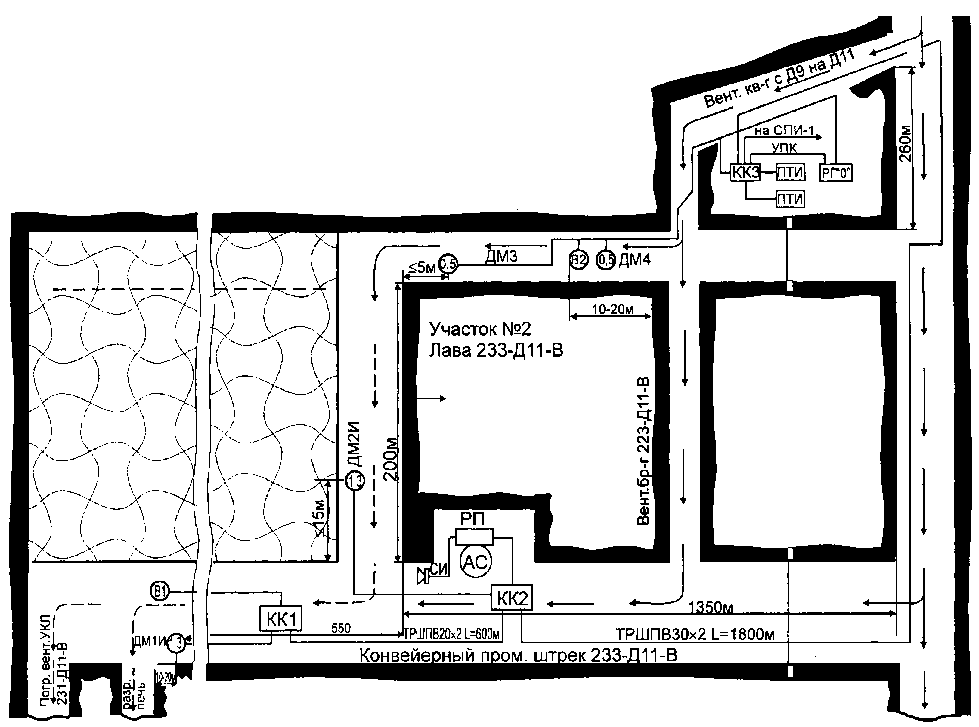
\includegraphics[width=0.8\textwidth]{image72}
    \caption*{Сурет 4 - Датчиктердің №2 өндіру учаскесінде орналасуы}
\end{figure}
\begin{figure}[H]
    \centering
    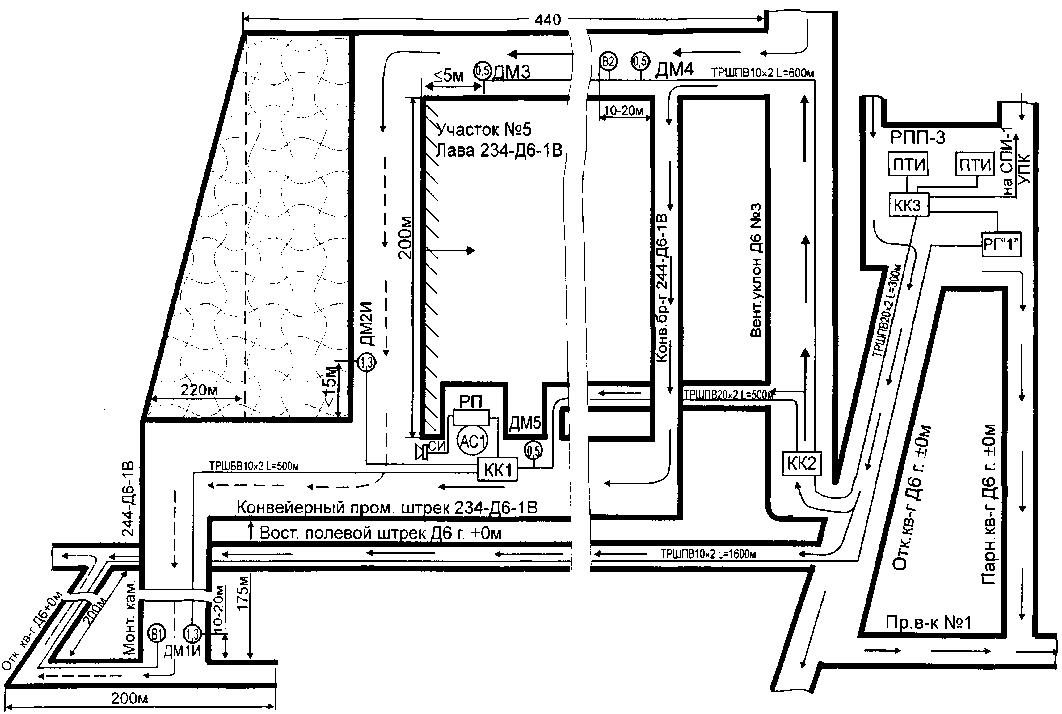
\includegraphics[width=0.8\textwidth]{image73}
    \caption*{Сурет 5 - Датчиктердің № 5 өндіру учаскесінде орналасуы}
\end{figure}

\begin{multicols}{2}
{\bfseries Алынған деректерді талқылау.} Автоматика және телеметрия
жүйесінің элементтерін орналастырудың ұсынылған жобасының жаңалығын
ескере отырып, алынған нәтижелер практикалық растауды қажет ететінін
түсіну қажет. Автоматика мен телемеханиканың бүкіл жүйесі сыналған нақты
жағдайлар да маңызды рөл атқарады.

{\bfseries Қорытынды.} Осылайша, ұйымдастырушылық және регламенттеуші
құжаттарды енгізумен бірге "Қазақстан" шахтасында диспетчерлендіру және
бақылауды автоматтандыру жобасын іске асыру өте маңызды нәтижелерге қол
жеткізуге мүмкіндік береді. Оларға шахта қауіпсіздігінің жаңа жоғары
деңгейіне шығу, Төтенше жағдайлар мен жабдықтардың тоқтап қалуы,
шығындарды азайту және шығындарды азайту жатады. Сондай-ақ, бұл
өнеркәсіптік қауіпсіздікті, штаттан тыс және авариялық жағдайларды жою
мерзімдерін қысқартуды, кәсіпорынды басқарудың сапасы мен жеделдігін
арттыруды және жедел және қызмет көрсететін персоналды оңтайландыруды
қамтамасыз етуге мүмкіндік береді.
\end{multicols}

\begin{center}
{\bfseries Әдебиеттер}
\end{center}

\begin{enumerate}
\item
Трубецкой К.Н., Кулешов А.А., Клебанов А.Ф., Владимиров Д.Я.
"Современные системы управления горно-транспортными комплексами". М.:
Недра.2014. - 263 с.

\item
Овсянников Ю.А., Кораблев В.А. Автоматизация подземного оборудования.
М.: Недра.2012. - 297 с.

\item
Портнов В.С., Юров В.М. Аппаратура диспетчеризации горного
оборудования. КарПТИ. 2009. Караганда. 2013. - 281 с.
\end{enumerate}

\begin{center}
{\bfseries References}
\end{center}

\begin{enumerate}
\item
Trubetskoy K.N., Kuleshov A.A., Klebanov A.F., Vladimirov D.Ya.
"Modern management systems of mining and transport complexes". M:.
Nedra. 2014. 263 p.

\item
Ovsyannikov Yu.A., Korablev A.A. Automation of underground equipment.
M:. Nedra. 2012. 297 p.

\item
Portnov V.S., Yurov V.M. Equipment for dispatching mining equipment.
CarPTI. 2009. Karaganda. 2013. - 281 c.
\end{enumerate}

\emph{{\bfseries Авторлар туралы мәліметтер}}

\begin{itemize}
\item
Тулегулов Амандос Дабысұлы - физика-математика ғылымдарының кандидаты,
қауымдастырылған профессор, кафедра меңгерушісі, Қазақ технология және
бизнес университеті, Астана, Қазақстан, tad62@ya.ru;

\item
Акишев Каршыга Мақсұтұлы, техника ғылымдарының кандидаты,
қауымдастырылған профессор. Қазақ технология және бизнес университеті,
Астана. Қазақстан,
akmail04@gmail.com

\item
Юрков Николай Кондратьевич, техника ғылымдарының докторы, профессор.
Пенза мемлекеттік университеті, Пенза, Ресей,
nk49@mail.ru

\item
Дмитрий Островерхов. Зерттеу инженері. Берлин техникалық университеті,
Берлин, Германия, tub14@mail.ru
\end{itemize}

\emph{{\bfseries Information about the authors}}

\begin{itemize}
\item
Tulegulov Amandos Dabysovich, Candidate of Physical and Mathematical
Sciences, Associate Professor, Head of the Department. Kazakh University
of Technology and Business, Astana, Kazakhstan, tad62@ya.ru;

\item
Akishev Karshiga Maksutovich, Candidate of Technical Sciences, Associate
Professor, Kazakh University of Technology and Business, Astana,
Kazakhstan.
akmail04@gmail.com

\item
Yurkov Nikolay Kondratievich, Doctor of Technical Sciences, Professor,
Penza State University, Penza,Russia. nk49@mail.ru

\item
Ostroverkhov Dmitry - Research engineer, Berlin Technical University,
Berlin, Germany, tub14@mail.ru
\end{itemize}
